\documentclass[tikz, border=5mm]{standalone}
\usepackage{amsmath} % For \text command in math mode
\usetikzlibrary{arrows.meta, positioning, decorations.pathreplacing, shapes.symbols}

\begin{document}

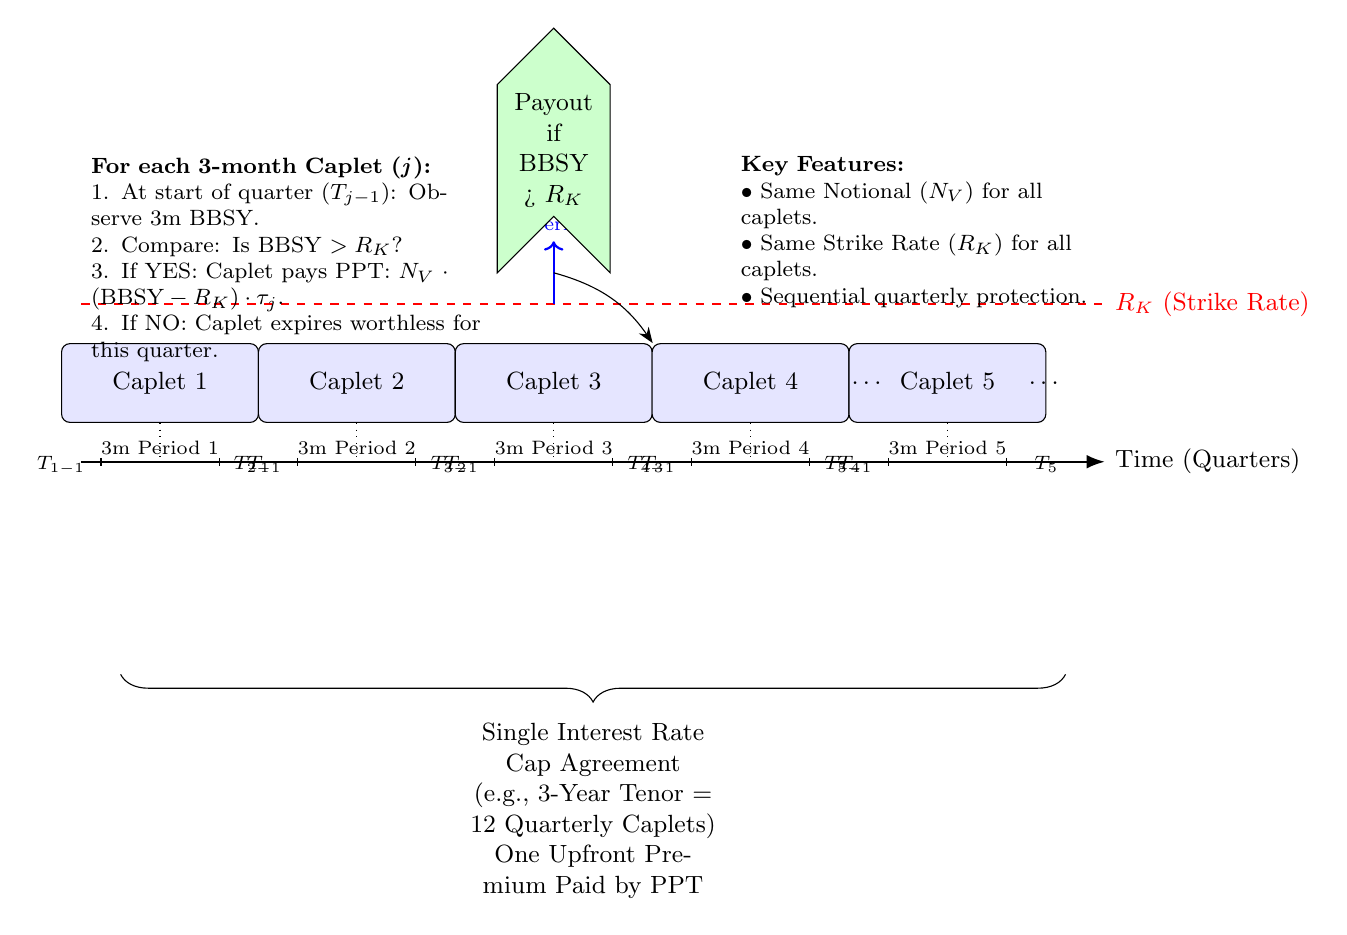
\begin{tikzpicture}[
    font=\small,
    node distance=0.7cm and 1.5cm,
    caplet/.style={rectangle, draw, fill=blue!10, minimum height=1cm, minimum width=2.5cm, text centered, rounded corners=3pt},
    timeline/.style={-Latex, thick},
    strike/.style={dashed, red, thick},
    payout/.style={signal, signal from=south, signal to=north, draw, fill=green!20, minimum height=0.6cm, text width=1.2cm, align=center},
    period_label/.style={font=\scriptsize, below=0.1cm of #1},
    time_label/.style={font=\scriptsize, below=0.3cm of #1}
]

% Timeline
\draw[timeline] (0,0) -- (13,0) node[right, font=\small] {Time (Quarters)};

% Overall Cap Agreement
\draw[decorate, decoration={brace, amplitude=10pt, mirror, raise=2.5cm}]
    (0.5,-0.2) -- (12.5,-0.2) node[midway, below=3cm, align=center, text width=5cm]
    {Single Interest Rate Cap Agreement \\ (e.g., 3-Year Tenor = 12 Quarterly Caplets) \\ One Upfront Premium Paid by PPT};

% Strike Rate Line
\draw[strike] (0,2) -- (13,2) node[right, font=\small, color=red] {$R_K$ (Strike Rate)};

% Caplets
\foreach \i [count=\quarter from 1, evaluate=\quarter as \labelQ using int(\quarter)] in {1, 3.5, 6, 8.5, 11} { % Positions for 5 example caplets for a 3-year cap
    \pgfmathsetmacro{\qtr}{\labelQ}
    \pgfmathsetmacro{\nextqtr}{int(\qtr+1)}
    \pgfmathsetmacro{\nodeX}{\i} % X position of the caplet node

    % Caplet Box
    \node[caplet] (caplet\qtr) at (\nodeX,1) {Caplet \labelQ};
    \node[period_label=caplet\qtr, text width=2cm, align=center] {3m Period \labelQ};
    \node[time_label=caplet\qtr.south west] {$T_{\labelQ-1}$}; % Start of period
    \node[time_label=caplet\qtr.south east] {$T_{\labelQ}$};   % End of period

    % Connection to timeline (visual)
    \draw[dotted] (caplet\qtr.south) -- (\nodeX,0);
    \draw (\nodeX-0.75, 0.05) -- (\nodeX-0.75, -0.05); % Tick for start of period
    \draw (\nodeX+0.75, 0.05) -- (\nodeX+0.75, -0.05); % Tick for end of period

    % Illustrative BBSY and Payout for one caplet (e.g., Caplet 3)
    \ifnum\qtr=3
        \draw[blue, thick, ->] (\nodeX, 2) -- (\nodeX, 2.8) node[above, font=\scriptsize, align=center] {3m BBSY \\ for Period 3};
        \node[payout, above=0.1cm of caplet\qtr, xshift=0cm, yshift=1.5cm] {Payout if \\ BBSY > $R_K$};
        \draw[-{Stealth[length=2mm, width=1.5mm]}] (\nodeX, 2.4) to[bend left=20] (caplet\qtr.north east); % Arrow to payout
    \fi
}

% Dots for continuation
\node at (10,1) {\dots}; % Indicating more caplets
\node at (12.25,1) {\dots};

% Labels & Annotations
\node[align=left, text width=5cm, anchor=north west, font=\footnotesize] at (0,4) {
    \textbf{For each 3-month Caplet (\textit{j}):} \\
    1. At start of quarter ($T_{j-1}$): Observe 3m BBSY. \\
    2. Compare: Is BBSY $> R_K$? \\
    3. If YES: Caplet pays PPT: $N_V \cdot (\text{BBSY} - R_K) \cdot \tau_j$. \\
    4. If NO: Caplet expires worthless for this quarter.
};

\node[align=left, text width=4.5cm, anchor=north east, font=\footnotesize] at (13,4) {
    \textbf{Key Features:} \\
    $\bullet$ Same Notional ($N_V$) for all caplets. \\
    $\bullet$ Same Strike Rate ($R_K$) for all caplets. \\
    $\bullet$ Sequential quarterly protection.
};

\end{tikzpicture}

\end{document}